%% LaTeX template for BSc Computing for Games final year project dissertations
%% by Edward Powley
%% Games Academy, Falmouth University, UK

%% Based on:
%% bare_jrnl.tex
%% V1.4b
%% 2015/08/26
%% by Michael Shell
%% see http://www.michaelshell.org/
%% for current contact information.
%%
%% This is a skeleton file demonstrating the use of IEEEtran.cls
%% (requires IEEEtran.cls version 1.8b or later) with an IEEE
%% journal paper.
%%
%% Support sites:
%% http://www.michaelshell.org/tex/ieeetran/
%% http://www.ctan.org/pkg/ieeetran
%% and
%% http://www.ieee.org/

%%*************************************************************************
%% Legal Notice:
%% This code is offered as-is without any warranty either expressed or
%% implied; without even the implied warranty of MERCHANTABILITY or
%% FITNESS FOR A PARTICULAR PURPOSE! 
%% User assumes all risk.
%% In no event shall the IEEE or any contributor to this code be liable for
%% any damages or losses, including, but not limited to, incidental,
%% consequential, or any other damages, resulting from the use or misuse
%% of any information contained here.
%%
%% All comments are the opinions of their respective authors and are not
%% necessarily endorsed by the IEEE.
%%
%% This work is distributed under the LaTeX Project Public License (LPPL)
%% ( http://www.latex-project.org/ ) version 1.3, and may be freely used,
%% distributed and modified. A copy of the LPPL, version 1.3, is included
%% in the base LaTeX documentation of all distributions of LaTeX released
%% 2003/12/01 or later.
%% Retain all contribution notices and credits.
%% ** Modified files should be clearly indicated as such, including  **
%% ** renaming them and changing author support contact information. **
%%*************************************************************************


\documentclass[journal]{IEEEtran}

\usepackage{graphicx}
% Insert additional usepackage commands here
\usepackage[hyphens]{url} % <===========================================
\usepackage[hidelinks]{hyperref} % Allows clickable reference lists
\usepackage[none]{hyphenat} %Stops breaking up words in table
\usepackage{cite}
\usepackage{listings}
\usepackage{amssymb}
\usepackage{upgreek}
\usepackage{siunitx}

\usepackage[table,pdftex,dvipsnames]{xcolor} 

\begin{document}
%
% paper title
% Titles are generally capitalized except for words such as a, an, and, as,
% at, but, by, for, in, nor, of, on, or, the, to and up, which are usually
% not capitalized unless they are the first or last word of the title.
% Linebreaks \\ can be used within to get better formatting as desired.
% Do not put math or special symbols in the title.
\title{ How Will a Mixed-Initiative Level Editor that Predicts User Requirements Affect the Levels Created?}
%
%
% author name

\author{Tristan Barlow-Griffin}

% The paper headers -- please do not change these, but uncomment one of them as appropriate
% Uncomment this one for COMP320
\markboth{COMP320: Research Review and Proposal}{COMP320: Research Review and Proposal}
% Uncomment this one for COMP360
% \markboth{COMP360: Dissertation}{COMP360: Dissertation}

% make the title area
\maketitle

% As a general rule, do not put math, special symbols or citations
% in the abstract or keywords.
\begin{abstract}
Mixed-initiative systems are becoming more affluent both within and outside of the gamed industry. These mixed-initiative systems are taking an ever-increasing number of different roles; from generating entire levels to fostering creativity in game designers. With the increasing cost of game development having a tool that can help to quickly and effectively prototype levels will reduce the costs of development significantly.
User feedback from a study on a mixed-initiative level designer requested a feature that will reduce the number of clicks required when designing a level\cite{alvarez2018fostering}. Predictive texting settings are available with almost every smartphone available to purchase. This feature aims to reduce the number of clicks required to create a word by predicting the word the user wishes to type.
This paper will discover if implementing a mixed-initiative component that aims to emulate predictive texting but in a level design context, will solve the feature requested in \cite{alvarez2018fostering}. Further research will look into whether this component will produce results similar to findings in existing predictive texting literature. Finally, there will be research into whether this component may cause the users to consider different level designs when the component takes a more proactive role in the creation process.

\end{abstract}

\markboth{COMP320: Research Review and Proposal}{COMP320: Research Review and Proposal}

\section{Introduction} \label{intro}
\IEEEPARstart{T}{his} research project will look into how a prototyping tool with a Mixed-Initiative (MI) component that predicts user requirements will affect the process and design of a level. A prototype is the initial design of an object \cite{prototype}, the prototyping phase is used to quickly test certain aspects of a products' design so the designer can identify and clear up any problems before full production commences\cite{budde1992prototyping}. Fullerton \textit{et all} \cite[p.~150]{fullerton2004game} state there are two kinds of prototyping in games: Physical and Software prototypes. Since the books publication in 2004, the accessibility of tools that help designers prototype levels has increased. Fullerton \textit{et al} \cite[p.~164]{fullerton2004game} also describes a level editor as a good way to prototype levels. The free to download game engine called \textit{Unreal Engine 4} (UE4) has a level editor built into it. Within this editor, the designers can create basic geometry scaling them to fit their needs. In addition, designers can add custom meshes and programmable objects to turn their levels into games.

The prototyping phase is meant to test the design of a product, the less time and resources required to produce an artefact that can demonstrate the proposed design the better. Beyond the benefit of saving time, the less time a designer puts into a particular design the less attached to the design they become. When collaborating in a group, differing opinions can cause different constraints to be set on the design of a product. While a given design may satisfy the original designers set constraints, the prototype may have to be discarded as it did not meet the other requirements set by the team. Identifying and discarding concepts early in development can save a lot of time and energy \cite[p.489]{stempfle1999thinking}. Arguably, this will reduce the negative impacts to interpersonal relations that idea dismissal may have. Developing a level editor that is meant to only prototype a levels' design will allow for less focus on the polish of the level created as the aim of the prototype is just to test if it fits the users requirements. This paper will build upon a standard level editor by adding an MI component, this component aims to implement features requested from Alvarez \textit{et al}\cite{alvarez2018fostering} study on their MI level editor. The implementation of these features is meant to increase the overall ease of designing a level through predicting what the user may require. In addition, this paper looks at the Sentient Sketchpad\cite{liapis2013sentient} an existing MI level editor, comparing their design to MI tool design theory and general user interface (UI) design theory. The hypotheses in this paper are only concerned with how the MI component interacts with the participants and what kind of impact theses interactions will have when trying to prototype a level. Looking at existing studies on the most effective prediction methods \cite{shepperd2001comparing,mendes2002further, wen2012systematic} this paper identifies and evaluates the methods proposed in the context of a MI level editor.  

\section{Related Work}
The lack of documentation about prediction methods being used in game design, required this paper to go  beyond the scope of just game design examples. The methods of prediction used in this study must be effective for the hypotheses to be tested accurately. To this end, Section~\ref{prediction} looks at currently used prediction methods comparing the performance results of each method. In Section~\ref{MI}, mixed-Initiative tools are group into two broad categories using Liapis~\textit{et al}\cite{liapis2016mixed} definition. The definition of mixed-initiative used in this paper will also be defined in Section~\ref{MI}. Defining these groups makes it easier to distinguish between the most common types of mixed-initiative tools. This section will also explore the different ways MI tools are being leveraged both within and outside of the games industry. In Section~\ref{UI} there is an evaluation of the existing mixed-initiative level editors. There is also a discussion and comparisons of these MI editors in the context of more general MI and UI design theory.  

\section{Mixed-initiative} \label{MI}
The term mixed-initiative was first introduced in \textit{1970} by Jaime R \cite{carbonell1970mixed}.
It describes a process whereby a computer and a human designer work together to achieve a goal. Other definitions of mixed-initiative build on the idea of human-computer co-creativity. This paper will use the first definition of mixed-initiative presented, as trying to define creativity is a very complex matter in itself. 

There are two broad categories that MI tools can be grouped into, Interactive evolution and Computer-aided design \cite{liapis2016mixed}. 
\begin{itemize}
    \item \textit{Interactive evolution}(IE) is where the designer has the idea, and the computer helps them realise it. The computers' role is to evaluate the humans' design, presenting alternative solutions if any constraints are broken. 
    
    \item \textit{Computer-aided design} (CAD) is where the computer generates the content, but does not evaluate the quality of the produced work. In CAD, the human designer will evaluate the work and use these evaluations to move towards a more desirable product space.
\end{itemize}

The first documented mixed-initiative tool created helped students to learn the English language\cite{carbonell1970mixed}. The uses of mixed-initiative tools have greatly expanded since 1970 and have been described as a backbone tool for designers \cite{alvarez2018fostering}. The application of mixed-initiative systems in more complex environments have given mixed results \cite{barnes2015designing}. Barnes \textit{et al}\cite{barnes2015designing} found that in most cases, systems that divide decision making between a human and an intelligent agent were generally more effective than if decisions were just dependent on the one. This can be seen with predictive texting, only choosing the words suggested to you by your phone can result in unexpected and hilarious results \cite{quicktype}. Barnes \textit{et al}\cite{barnes2015designing} found that human designers were better at making abstract decisions and inferring the significance of an object or event. Kantosalo \textit{et al}\cite{kantosalo2014isolation} focus their MI tool on user-centred design, this means their AI agent played a back-seat role. Kantosalo \textit{et al}\cite{kantosalo2014isolation} propose future work where the agent and the designer have an equal role in the system, they do not make any conjecture on the anticipated results.

 PCG and CAD are closely related fields, the difference between CAD and PCG is in the evaluation period. If a designer were to use a PCG algorithm to generate a level and then look through the produced results evaluating and picking maps this would be considered CAD\cite{liapis2016mixed}. For it not to be considered CAD, the PCG algorithm would have to perform the evaluation itself. For example, this might include checking if the map is completable or if it is a certain size. The field of procedural content generation(PCG) has advanced significantly \cite{van2013designing}. The uses of PCG are ever increasing as publishers seek to lower costs of production\cite{doherty2005mixed, font2016constrained}.

One may choose to use PCG in games as it will increase the quantity and variation of levels produced ensuring replayability \cite{karavolos2015mixed}. PCG algorithms can also be shipped with the games they are made for, this allows for an inexhaustible source of new maps \cite{johnson2010cellular}. Doing so will extend the games life-span giving the players an amount of content that would otherwise be impossible. Although there is no guarantee that this content will be interesting or unique. However, using CAD tools to generate maps there will always be a human element evaluating the maps. With this input the human designer may discard maps that are similar to existing maps, thus providing quality assurance not present in a PCG algorithm.

Prototyping a level should be a fast iterative process \cite{smith2011tanagra}, the method used to prototype should allow for instant feedback on the design. This feedback needs to have an easy channel back to the designer so that amendments can be made with ease. Map generation algorithms, even in under ideal circumstance will only provide the designer with a set of parameters to change\cite{doran2010controlled}. Small variations in the given parameters can produce large changes in the maps design\cite{regier2009random}. This will make it difficult to make small changes when given feedback. As a result, reduce the effectiveness of a CAD approach when trying to prototype levels.

Within an IE environment, the core of the creative process relies on the human designer. As the main creative driver, the human has the most input. Ideally, the computer will add value by providing supplementary support, for example, alerting the designer when constraints have been broken. It can be argued as the constraints are determined more by the human, the size of the possible output space will be larger. Yanakakis \textit{et al} \cite{yannakakis2014mixed} claim that CAD examples like PCG limit the designers' intentions as they follow their own algorithms. Doran and Parberry\cite{doran2010controlled} inadvertently corroborate Yanakaki\textit{et al}\cite{yannakakis2014mixed} view, as they say, a PCG algorithm should ideally, have a set of designer-centric parameters as their only form of control. This limited control over the creation of levels may, in some situations, be enough. During the prototyping phase, when the requirements needed from a map are changing the fastest, the level of control provided through CAD might not be enough to handle large changes in design. 

\section{Mixed-Initiative Level Editors } \label{UI}
A user interface should be intuitive to use and not require any additional helping systems \cite{oppermann2002user}. Liapis \textit{et al} \cite{liapis2013sentient} aim to achieve this by creating a design tool that allows users to create levels using a low-resolution graphical interface. Figure~\ref{Sketchbook} shows the interface used to design levels for a strategy game. The designer can place tiles on the map which will colour in the given tile with the placed tiles colour. During a tile placement, the tool will test for the playability of the map, checking to see if placing the current tile will break any of the games' constraints. The Sentient sketchbook also provides alternative viewing modes, examples of these alternate viewing models can be seen in Figure~\ref{Sketchbook2}. There is no mention in the study how often these tools were used, Galtiz \cite[p.~752]{galitz2007essential} warns against too many graphics on the screen.

\begin{figure}[h]
	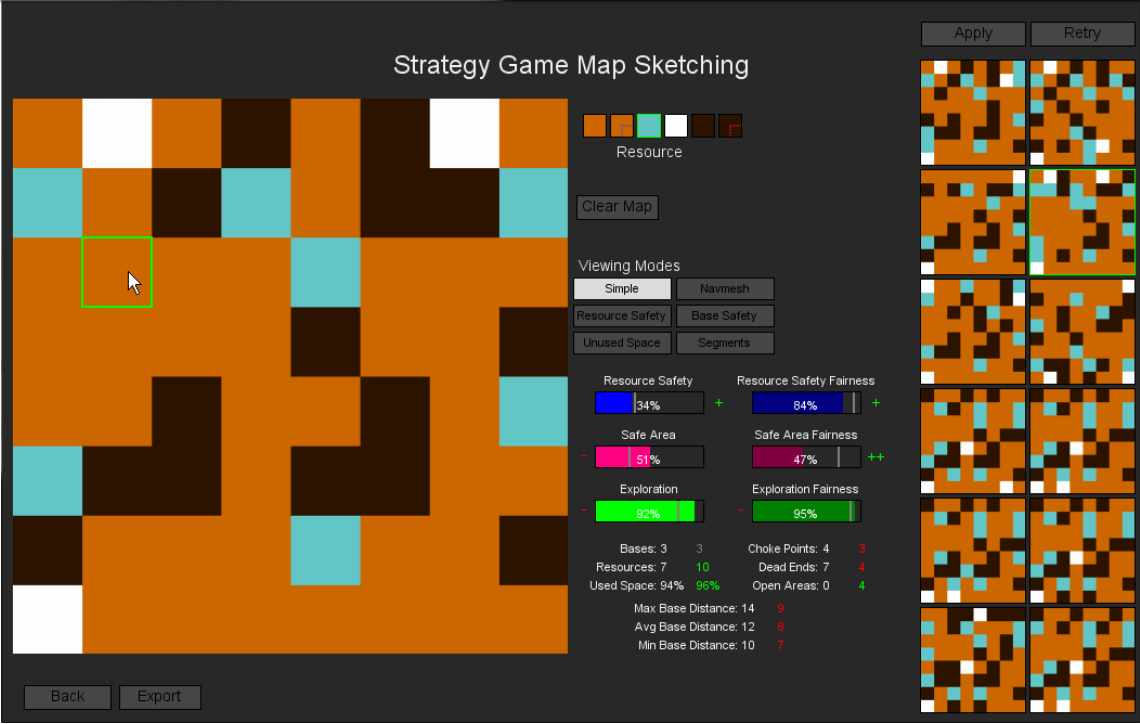
\includegraphics[width=1.0\linewidth]{SentientSketchbook.PNG}
	\caption{Liapis \textit{et al} Sentient Sketchbook during a design session ~\cite{liapis2013sentient}.}
	\label{Sketchbook}
\end{figure} 

\begin{figure}[h]
	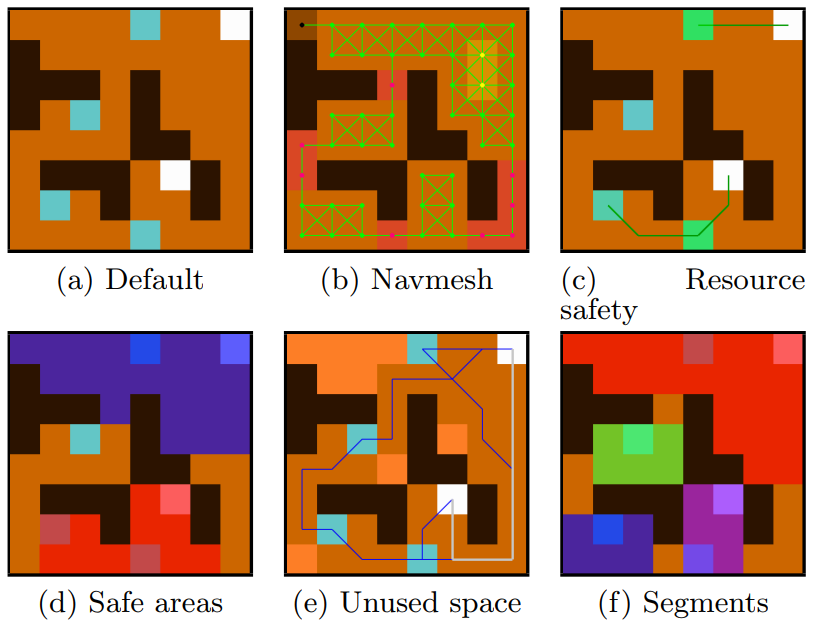
\includegraphics[width=1.0\linewidth]{SentientSketchbook2.PNG}
	\caption{Liapis \textit{et al} Sentient Sketchbook Different viewing modes ~\cite{liapis2013sentient}.}
	\label{Sketchbook2}
\end{figure} 

Baldwin \textit{et al} \cite{baldwin2017mixed} have also implemented a mixed-initiative dungeon designer called the evolutionary dungeon designer or (EDD) for short. EDD is closer to a CAD tool than the IE tool Sentient Sketchbook \cite{liapis2013sentient}. While the approaches may be different see Figure~\ref{EDD}, both MI tools allow for large customisation of the levels generated see Figure~\ref{EDD}. Baldwin \textit{et al} \cite{baldwin2017mixed} take a different approach to Liapis \textit{et al}\cite{liapis2013sentient}. Baldwin \textit{et al} \cite{baldwin2017mixed} core concept is to identify design patterns within the level design. These design patterns consist of multiple tiles that constitute common patterns found in games. Alvarez \textit{et al}\cite{alvarez2018fostering} builds upon the EDD suggested in \cite{baldwin2017mixed} by adding an IE element to it. It could be argued that the new version of the EDD has an improved interface with lots of its excess drop-down menus gone see Figure~\ref{EDD2}. Beyond the ascetic differences, Alvarez \textit{et al}\cite{alvarez2018fostering} dungeon designer integrates key aspects of the Sentient Sketchpad \cite{liapis2013sentient}. The second edition of the EDD allows the user to design their own levels, it will then offer suggestions based upon the map the user created, this can be seen in the top right corner of figure~\ref{EDD2}. The results from Alvarez \textit{et al}\cite{alvarez2018fostering} experiment focused on whether their tool fostered creativity in the participants using it. Included with the results is a table of requested features made by the participants of the study. One key element highlighted is that the EDD should do a ``bit more automated assistance when doing manual designs, which can reduce clicking around the program" \cite[Table 2]{alvarez2018fostering}. Another significant feature request was for the dungeon designer to take into account the pattern of the entire dungeon, using the map of the dungeon to generate new rooms.

\begin{figure}[h]
	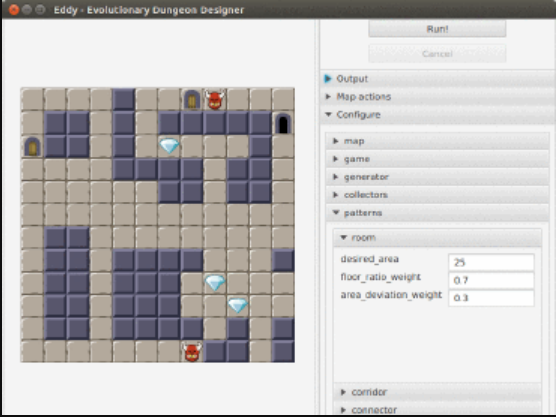
\includegraphics[width=1.0\linewidth]{EDD.PNG}
	\caption{ Baldwin \textit{et al} Evolutionary Dungeon Designer user interface ~\cite{baldwin2017mixed}.}
	\label{EDD}
\end{figure} 

\begin{figure}[h]
	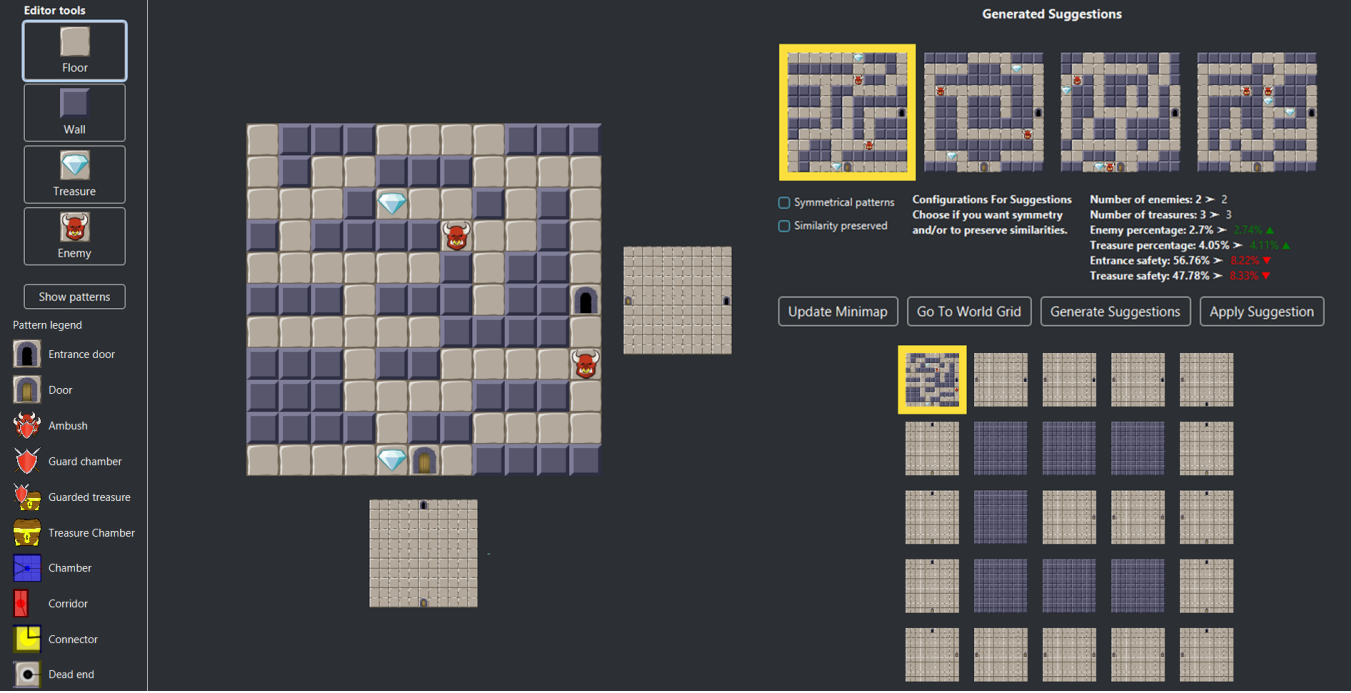
\includegraphics[width=1.0\linewidth]{EDD2.PNG}
	\caption{ Alvarez \textit{et al} Evolutionary Dungeon Designer with modifications user interface ~\cite{alvarez2018fostering}.}
	\label{EDD2}
\end{figure} 

Horvitz \cite{horvitz1999principles} proposes 12 critical factors to take into consideration when making a mixed-initiative user interface. While Horvitz \cite{horvitz1999principles} focuses on a mixed-initiative assistant for Microsoft Outlook (emailing software) it can be argued that some of these factors are relevant for a level designer. The first factor that is listed is that an MI tool needs to add significant value through the automation of services. An example of a service automated by emailing assistant is the sorting of a users' emails into different categories. Within the context of \cite{liapis2013sentient} they satisfy \cite{horvitz1999principles} first critical factor by allowing the computer to automate some of the map design services like checking for broken game constraints. Liapis \textit{et al} \cite{liapis2013sentient} also allows their algorithm to take on a creative role all be it based on an original human designed map. Within this project, the focus will not be on the creative aspect as the definition of creativity is hard to for a computer to understand \cite{jordanous2010defining}. Alvarez \textit{et al}\cite{alvarez2018fostering} found their MI tool is better at providing controllability than expressivity, when the user imposes their vision, as it is hard for a computer to capture the designers' vision. It can be argued that an MI tool could not consistently add value if it cannot capture the designers' vision. Smith \textit{et al}\cite{smith2011tanagra} believe that human designers strengths lay in creativity and their ability to evaluate good content and the computer lacks this ability. 

Another factor raised by Horvitz \cite{horvitz1999principles} is that a tool must consider minimizing the costs of poor guesses about the users' goals. Even with an extensive history of the users' requirements, a novel use of the tool might be required. It is important for a system to recognise when something novel is happening and for it not to attempt predictions. Some authors find value in these missed guesses and even seek to find novelty search spaces \cite{liapis2013sentient}. Other authors \cite{liapis2016can,alvarez2018fostering, yannakakis2014mixed} claim these kind of mistakes can foster creativity and alternate suggestions that do not aim to predict the user can be beneficial. On the right-hand side of Figure~\ref{Sketchbook} the results of the guessing algorithm are shown. Clicking retry will remove the current maps and create new ones for the designer to evaluate.

None of the above examples \cite{alvarez2018fostering, liapis2013sentient, baldwin2017mixed} satisfy Barnes \textit{et al}\cite{barnes2015designing} statement that an MI systems UI must provide transparency to the reasoning behind the agents actions. In all cases above\cite{alvarez2018fostering, liapis2013sentient, baldwin2017mixed} , when generating new suggestions the reasoning behind each suggestion was not given to the designer. The designer is presented with the statistics of the current map generated (density, number of resources etc.) but it is not clear from the interface how these statistics are being used. Lee and See\cite{lee2004trust} agrees with Barnes \textit{et al}\cite{barnes2015designing} that MI systems should be transparent, they go so far as to say it is required for a human to trust the automation process \cite{lee2004trust}.

\section{Prediction Methods} \label{prediction}
Predictive texting increases the average message length users send to each other \cite{ling2005length} as well as the speed the words are written \cite{dunlop2000predictive}. The same theory may apply to game design. If patterns of a users game design are established, an AI system may be able to assist in design. In this section, this paper will look into different methods of predicting human requirements, this paper will also discuss the pros and cons of each technique.

The researchers of \cite{chipalkatty2013less} have tested alternate methods for predicting human input so as to abstract the low-level movements of the robots the humans were controlling. They built on the idea that humans are good for high-level abstract tasks, but an AI agent was much better at performing low-level repetitive control tasks. In addition, they found that when trying to predict the next human input, trying to identify patterns in a history of events was not successful. Instead, using just the last event yielded much better results, hence their title ``less is more". Instead of using current human inputs, \cite{bhatia2016targeted} used the history of the users' social media page to predict the users' interests. Perhaps if the authors of \cite{chipalkatty2013less} had looked less at the input history of the human and instead focused on grouping inputs together to create larger actions. Similar, to how modern day phones often predict entire sentences rather than just single words.

\subsection{Markov Chains}
Markov Chains implements a theory similar to the methods previously discussed by Bhatia and Hasija \cite{bhatia2016targeted}. A Markov chain is a special kind of process that works under the assumption that the state at time \textit{t+1} depends only on the current state. Another explanation is the state at time \textit{t+1} is exclusively dependent on the state at time \textit{t}. This means State \textit{t+1} is not dependent on the history of the states leading up to it\cite{ye2000markov}. This technique has been proven useful for predicting anomalies in systems \cite{ju2001hybrid, gwadera2005markov, ye2000markov} where the states are heavily dependent on the latter state happening. However, it is hard to see how during a creative process, where the next state is dependent on the vision of the designer, the state at \textit{t+1} can be predicted from just knowing the state at \textit{t}. 
The introduction of a Markov model makes Markov Chains method more viable as a prediction technique. A Markov model can be used to describe the probabilistic relationship between the previous states in a Markov Chain\cite{markov1971extension}. Higher order Markov chains relax the rule of the next state being only dependent on the current state by allowing the network structure to look \textit{n} number of states back from the current state\cite{ching2008higher}. Snodgrass and Ontanon\cite{snodgrass2017learning} used Markov models as a way to model level data. Using these Markov models Snodgrass \textit{et al}\cite{snodgrass2017learning} applied different sampling techniques, they found using their higher order Markov chains was more effective than using standard Markov chains. This conflicts with Chipalkatty \textit{et al}\cite{chipalkatty2013less} findings of ``less is more", Snodgrass and Ontanon\cite{snodgrass2017learning} found that using a history of states to predict the next state was more effective to achieve their goals.

\subsection{Artifical Neural Network}
An artificial neural network (ANN) consists of many nodes that are divided into separate layers. Each node receives inputs from other nodes, the value of these inputs depends on the weight of the connection between the nodes \cite{lai2010prediction}. ANN are used in prediction methods focusing on outputting numerical values \cite{lai2010prediction, akdag2009estimation}. Shepperd and Kadoda \cite{shepperd2001comparing} found that case-based reasoning(CBR) outperformed a ANN on more occasions. However, Shepperd and Kadoda\cite{shepperd2001comparing} highlighted the dependence of the respective techniques on the nature of the training sets used. Figure~\ref{learningSets} shows stepwise regression procedure proving to be more accurate at prediction than both CBR and ANN on small datasets. A time series approach to neural networks has been found to increase their accuracy when dealing with world state predictions \cite{hazarika1998neural}. The number of data points in the training set that Hazarika and Lowe\cite{hazarika1998neural} used was much larger than in \cite{shepperd2001comparing} at 500 points for training and 250 for validation. Looking at examples from \cite{liapis2013sentient, alvarez2018fostering,  baldwin2017mixed} the maximum level dimensions are 12 tiles wide by 12 tiles tall. This means that the maximum number of data points provided by one map would be 124, which is far less than Hazarika and Lowe\cite{hazarika1998neural} use to train their ANN.

\begin{figure}[h]
	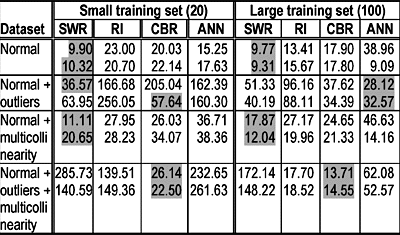
\includegraphics[width=1.0\linewidth]{trainingSets.PNG}
	\caption{Shepperd \textit{et al} Analysis of Accuracy (MMRE) for Continuous Model (Y1) ~\cite{shepperd2001comparing}.}
	\label{learningSets}
\end{figure} 

\subsection{Case-based Reasoning and Stepwise Regression procedure}
Case-based reasoning (CBR) is a prediction technique that uses a history of completed products to predict solutions to problems in the current product. This is done by comparing features in the current problem description to problems already solved in existing projects. Usually the problem description that is most similar to the current problem is used to estimate the solution\cite{watson1998applying, mendes2002further}. The core of a case -based reasoner is solving new problems by using or adapting solutions from old problems \cite{riesbeck2013inside}. Watson \cite{watson1999case} describes CBR as a methodology not a technique and provides several different techniques to apply CBR. Mendes and Mosley\cite{mendes2002further} have compared some of the techniques found in \cite{watson1999case} as well as additional techniques. They found that using a CBR technique that used adaptation rules performed significantly better than techniques that did not use adaption rules. In addition, they found the CBR techniques that used weighted euclidean distance also gave the best predictions. Much like Shepperd and Kadoda\cite{shepperd2001comparing}, Mendes and Mosely\cite{mendes2002further} also found that stepwise regression gave the best prediction accuracy ``for all measures of prediction accuracy'' \cite[p. 11]{mendes2002further}. The dataset used in \cite{mendes2002further} consisted of 34 data points which could be considered a small data set when comparing the number of data points used in \cite{hazarika1998neural}. Looking at Figure~\ref{learningSets}  there is a strong case for both SWR and CBR as prediction techniques with a small data set. Wen \textit{et al}\cite{wen2012systematic} also state CBR to be accurate with a small data sets ,validating the results found by Shepperd and Kadoda\cite{shepperd2001comparing}. If CBR is described as being accurate with a small data set \cite{wen2012systematic} and SWR techniques consistently out perform it with both small and large sets \cite{shepperd2001comparing,mendes2002further}it can be inferred that SWR is also a good technique to use with small data sets. 
Stepwise regression adds to the prediction model the variables with the highest partial correlation to the response variable at each stage\cite{schroeder2016understanding}. With the aim to have a set of variables (predictors) in the model to maximise \textit{F}, \textit{F} describes the association of all of the predictors to the response variable \cite{schroeder2016understanding}. For a variable to be added to the model it must increase \textit{F} by a constant specified amount \textit{a} commonly described as the(Alpha-To-Enter) value. Similarly for a value to be removed from the model it is measured by its reduction in F and is also compared against a constant described as the (Alpha-To-Leave).

\section{Methodology}
One key motivation for this experiment comes from Alverezs' \textit{et al}\cite{alvarez2018fostering} literature, in particular a users' feature request for more automated assistance with the aim to reduce clicking. To this end, this project proposes a tile based level editor which has a mixed-initiative component. The mixed-initiative component will reduce clicks by predicting what the users next action will be. In addition, this MI component will be used to discover if the predictive texting findings of Ling \cite{ling2005length} and Dunlop and Crossan\cite{dunlop2000predictive} are applicable to level design. The research question proposed in this project is: How Will a Mixed-Initiative Level Editor that Predicts User Requirements Affect the Levels Created? 

\subsection{Hypotheses}\label{Hypotheses}
When creating a level editor the aim is to increase the ease at which levels could normally be created. For the scope of this paper, the focus is on the MI component within the context of the editor, not the editor itself. Table ~\ref{hyp} shows the proposed hypotheses for this paper, it also shows from which source of data each hypothesis depends. Ling \cite{ling2005length} found that predictive texting increased the speed at which messages are written. Also, Dunlop and Crossan\cite{dunlop2000predictive} found that predictive texting also increased the size of the messages written. Hypothesis 2 and 1 will see if these findings are also applicable to level design with the MI component replacing the predictive texting element. Hypothesis 3 will be investigating whether a predictive component will satisfy the feature proposed by Alverezs' \textit{et al}\cite{alvarez2018fostering}. Hypothesis 4 will build on the work of Alvarez' \textit{et al}\cite{alvarez2018fostering} and see if the MI level editor can make designers consider alternative level design approaches. Finally, hypothesis 5 will discover if designers with more experience are more likely to find the MI a negative influence than designers with less experience, the argument being that more experienced designers do not need help to realise their design.

\begin{table*}[h]
		\centering
		\caption{Hypotheses Table}
		\label{hyp}
		\def\arraystretch{1.5}
		\begin{tabular}{|c|p{7cm}|p{7cm}|p{1.75cm}|}
			\hline
			& \textbf{Hypothesis}& \textbf{Null Hypothesis} & \textbf{Data Source}\\\hline
			1 & The MI component will effect the speed at which the participants create levels.
			& The MI component will not effect the speed at which the participants create levels.
			& Design Session Statistics\\ \hline
			
			2 & The MI component will effect the size of the levels the participants create.
			& The MI component will not effect the size of the levels the participants create.
			& Design Session Statistics\\ \hline

			3 & The MI component will effect the number of the clicks the designer makes.
			& The MI component will not effect the number of the clicks the designer makes.
			& Design Session Statistics\\ \hline

			4 & The MI component will influence participants to explore other level designs.
			& The MI component will not influence participants to explore other level designs.
			& Questionnaire\\ \hline

		          5 & The participants with more experience will be Negatively impacted more often by the MI component.
			&  There will be no correlation between experience and the negative impact of the MI component.
			& Questionnaire\\ \hline
			
		\end{tabular}
\end{table*}

\subsection{Participants}
Once a week, Falmouth Universities' Games Academy hosts different guild sessions for each game design route (design, art, animation, programming, writing and audio). All the participants for this experiment will be randomly sampled from these guild sessions through an online random name selector. Approaching the game design guild and another guild will ensure a range of level design ability.  
A power analysis for this experiment resulted in a sample size of 23. The power included a two-tailed t-test with an effect size of \textit{0.8}, an alpha error probability of \textit{0.05} and a \textit{power(1- beta error probability)} of \textit{0.95}. In this experiment all of the participants will be in one group, they will each be required to design levels using the level editor provided. By the end of the experiment, all of the participants will have designed the same number of levels. Everyone in this study will be asked to complete a consent form, given an information sheet and the option to quit the experiment at any time. The information sheet will only give the basic information of the project as we do not want to invite acquiescence bias\cite{watson1992correcting}. The data collected in this experiment will not be enough to identify anyone, keeping the participants anonymous.



\subsection{Design Session}
The design session will require the participants to create five different levels each with different editor settings. Before the session starts the users are prompted with a multiple choice question. This question will require the participants' to self-assess their own game design experience, from ``not a lot" to ``a lot" of design experience. After this, the user will be presented with the main level editor interface. They will then be given as much time as they need to familiarize themselves with the interface. The different editor settings the participants will be working in can be seen in Table~\ref{settings}. The order in which the different settings will occur will be random, this will reduce the impact of the practice effect on any data gathered. The computer will choose the order in which the editor setting will be applied. This means the observing researcher will not know what current settings are applied. By making this a double-blind study it will minimize the chance of investigator/observer bias \cite{phillips1999double}. Before each level starts an on-screen prompt will inform the user of the rules of the current level, for example: "During this level there will be a component that predicts your requirements.". All of the levels will be silently timed so as not to influence participants to work faster than they would usually. At any point during this experiment the participants can withdraw from the study, doing so will cause any data gathered on the levels they have created to be classified as incomplete and will be deleted. After completion of each level, the designer will be asked a few multiple choice questions. Each question will have five possible answers, the answers are relative to the questions asked but will follow a similar scale from negative to positive. After the questions have been answered any data gathered will be stored along with the current configuration. This will later be sent to the server once the participant has completed the experiment.
 The questions are:
\begin{itemize}
    \item How frequently did the level editor make you consider an alternative level design?
    
    \item How much impact did the level editor have on your work flow?

    \item What kind of impact did the level editor have on your work flow?

   \item How difficult did you find it to make the level you wanted?

    \item How pleased are you with the final design of the level?
\end{itemize}
An alternate method would be to have a questionnaire at the end of the experiment once all levels have been completed. However, as each set of responses correlates to a different editor configuration, it will make data management easier to get all the data for a single configuration in one go. In addition, leaving the questions until the end in one questionnaire may invite levelling and sharpening bias, this is where details are lost and others are heightened over time \cite{koriat2000toward}.

\begin{table}[h]
	\centering
	\caption{Editor Settings}
	\label{settings}
	\def\arraystretch{2}
\resizebox{\columnwidth}{!}{\begin{tabular}{|l|l|l|l|l|}
		\hline
		\textbf{Editor Settings} & \textbf{Predictive Placements Enables}& \textbf{Unrestricted size } & \textbf{Exploration}\\\hline
		Settings 1  &  X & X& \\ \hline
		Settings 2  &     & X &\\ \hline
		Settings 3  &   X&  &\\ \hline
		Settings 4  &    &  &\\ \hline
		Settings 5  & X &   & X\\ \hline
	\end{tabular}}
\end{table}

\subsection{The level editor}
In this experiment there will be two kinds of game objects that can be placed in the level rooms and props. Rooms will occupy tiles on the map, whereas the props can be placed within any of the rooms. Figure~\ref{myLevelEditor} shows the first prototype design for the level editor. Barnes \textit{et al}\cite{barnes2015designing} suggests that any mixed-initiative component should provide reasoning behind the agents actions, to do this the prototype contains an information log, this information log will be used to tell participants why the level editor has made a particular decision. The level view will be a tile based view of the current map, it will allow users to place tiles and props according to their respective rules. Figure~\ref{myLevelEditor} also shows the layout of the level editor, on the left is where the buttons to switch between what prop/room will be placed when the participant next clicks. The check button will be used to make sure the game is completable. The checking algorithm will be simple, it will make sure there is a start and an end tile, it will also check these tiles are connected by a valid path. The level complete button will perform a check before finishing to make sure a valid level is being submitted. If a level were to be rejected, the information log will be used to inform the user why it has been rejected.

\subsection{Prediction Technique}
When deciding the prediction technique for this experiment the main limiting factor to consider is the number data points available. In the MI level editors discussed in Section~\ref{UI},  the number of tiles present within a level did not exceed 144 \cite{alvarez2018fostering, liapis2013sentient, baldwin2017mixed}. By treating each tile as one data point this gives a maximum number of 144 data points to use when training the MI component. It has been proven that CBR techniques have proven to be effective at prediction even with a small data set \cite{shepperd2001comparing,wen2012systematic}. However, SWR has been proven to out perform CBR on multiple occasions \cite{shepperd2001comparing, schroeder2016understanding}. It seems clear that using a stepwise regression model will increase the accuracy of the MI component, allowing the focus to be on how the participants interact with the MI component and less on the accuracy of the predictions.

\begin{figure}[h]
	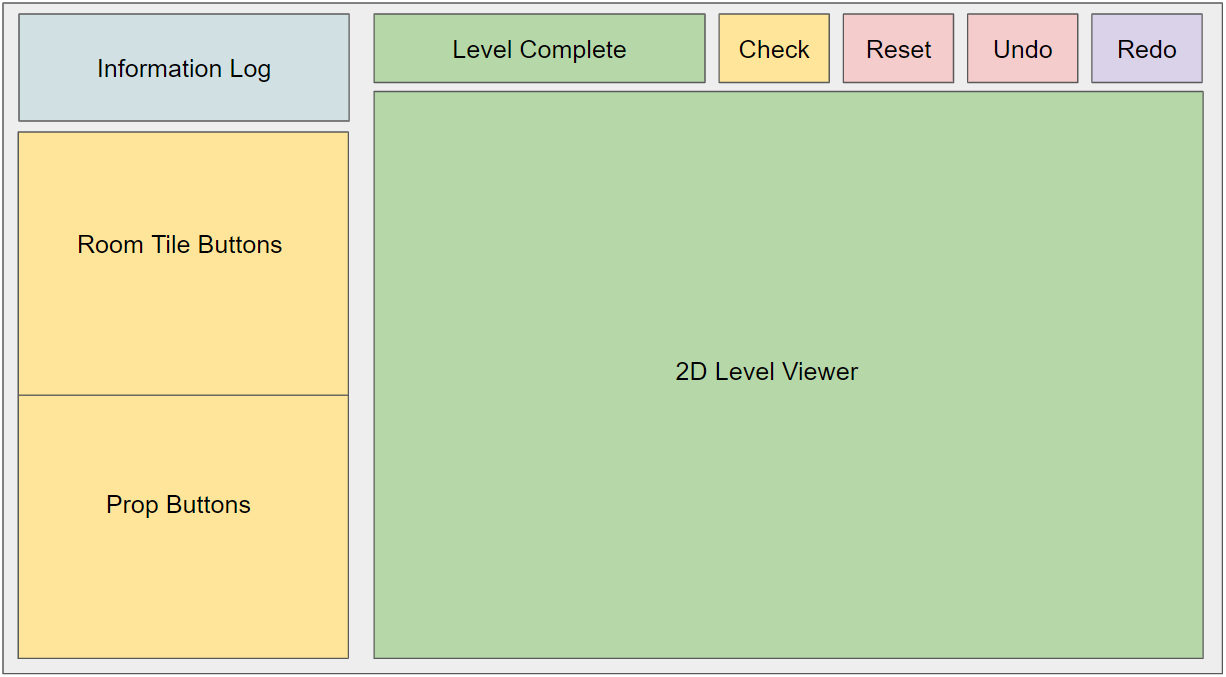
\includegraphics[width=1.0\linewidth]{LevelEditorLayout.PNG}
	\caption{The first iteration of the proposed level editor}
	\label{myLevelEditor}
\end{figure} 
\bibliographystyle{IEEEtran}
\bibliography{references}

% Appendices



% that's all folks
\end{document}
